% Manual of pgf-pie.sty, a convenient set of macros for drawing pie
% chart. Written by Xu Yuan <xuyuan.cn@gmail.com> This file is part of
% pgf-pie you may get it at http://code.google.com/p/pgf-pie/

\documentclass{article}
\usepackage[margin=12mm]{geometry}
\usepackage{hyperref}

\usepackage{pgf-pie}
\usetikzlibrary{shadows}

%%%%%%%%%%%%%%%%%%%%%%%%%%%%%%%%%%%%%%%%%%%%%%%%%%%%%%%%%%%%%%%%%
\usepackage{listings}
\usepackage{color}
\definecolor{listinggray}{gray}{0.92}
\lstset{ %
language=[LaTeX]TeX,
breaklines=true,
frame=single,
% frameround=tttt,
basicstyle=\footnotesize\ttfamily,
backgroundcolor=\color{listinggray},
keywordstyle=\color{blue}
}
%%%%%%%%%%%%%%%%%%%%%%%%%%%%%%%%%%%%%%%%%%%%%%%%%%%%%%%%%%%%%%%%%

%%%%%%%%%%%%%%%%%%%%%%%%%%%%%%%%%%%%%%%%%%%%%%%%%%%%%%%%%%%%%%%%%
\hypersetup{
  colorlinks=true,
  linkcolor=blue,
  anchorcolor=black,
  citecolor=olive,
  filecolor=magenta,
  menucolor=red,
  urlcolor=blue
}
%%%%%%%%%%%%%%%%%%%%%%%%%%%%%%%%%%%%%%%%%%%%%%%%%%%%%%%%%%%%%%%%%

%%%%%%%%%%%%%%%%%%%%%%%%%%%%%%%%%%%%%%%%%%%%%%%%%%%%%%%%%%%%%%%%%
\newcommand{\demo}[2][1]{
  \begin{center}
  \begin{tabular}{cc}
    \begin{minipage}{.49\linewidth}
      \centering
      \resizebox{#1\linewidth}{!}{
        \input{demo/#2}
      }
    \end{minipage}
    &
    \begin{minipage}{.45\linewidth}
      \lstinputlisting{demo/#2}
    \end{minipage}
  \end{tabular}
  \end{center}
}
%%%%%%%%%%%%%%%%%%%%%%%%%%%%%%%%%%%%%%%%%%%%%%%%%%%%%%%%%%%%%%%%%

%%%%%%%%%%%%%%%%%%%%%%%%%%%%%%%%%%%%%%%%%%%%%%%%%%%%%%%%%%%%%%%%%
\newcommand{\example}[2][1]{
  \begin{center}
    \resizebox{#1\linewidth}{!}{
      \input{demo/#2}
    }
  \end{center}
  \lstinputlisting{demo/#2}
}
%%%%%%%%%%%%%%%%%%%%%%%%%%%%%%%%%%%%%%%%%%%%%%%%%%%%%%%%%%%%%%%%%

\begin{document}
%%%%%%%%%%%%%%%%%%%%%%%%%%%%%%%%%%%%%%%%%%%%%%%%%%%%%%%%%%%%%%%%%
\title{Drawing Pie Chart by using \texttt{pgf-pie}}
\author{\href{mailto:xuyuan.cn@gmail.com}{Yuan Xu}}
\date{\today{}~(v0.2)}
\maketitle
%%%%%%%%%%%%%%%%%%%%%%%%%%%%%%%%%%%%%%%%%%%%%%%%%%%%%%%%%%%%%%%%%

\begin{abstract}
  \texttt{pgf-pie} is a LaTeX package for drawing pie chart (and
  variant charts). As stated by its name, it is based on a very
  popular graphic package \texttt{PGF/TikZ}. This document presents
  the usage of \texttt{pgf-pie} and collects some pie charts as
  examples. \texttt{pgf-pie} can be downloaded from
  \href{http://code.google.com/p/pgf-pie/}{http://code.google.com/p/pgf-pie/}.
\end{abstract}

\tableofcontents

\section{Usage}

\subsection{First Pie}
\lstinline|\pie| is the only coomand that provided by
\texttt{pgf-pie}. The argument is a list of number and text
combination in the formate of \texttt{number/text}, i.e. \texttt{10/A,
  20/B, 30/C, 40/D}. The result is shown in figure \ref{fig:first-pie}.
\begin{figure}
  \centering
  \demo[0.6]{first-pie}
  \caption{The first pie.}
  \label{fig:first-pie}
\end{figure}

\subsection{Position, Rotation, Size}

The center of chart can be set by \texttt{pos}, default is
\texttt{\{0,0\}}. The chart can be rotated by setting \texttt{rotate}
(in degrees). The size of chart can be set by \texttt{radius}, default
is 3.

\demo{radius}

\subsection{Color}
The color can be specified by \texttt{color}, the default color wheel
is shown in figure \ref{fig:color-wheel}.
\begin{figure}
  \centering
  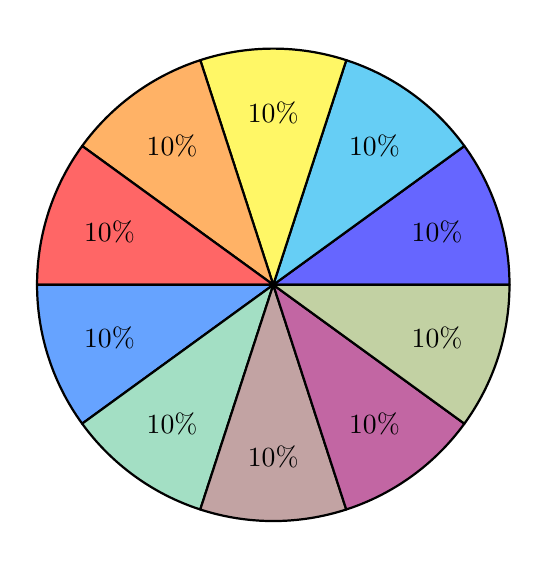
\begin{tikzpicture}
  \pie{10/, 10/, 10/, 10/, 10/, 10/, 10/, 10/, 10/, 10/}
\end{tikzpicture}
  \caption{Default color wheel}
  \label{fig:color-wheel}
\end{figure}

\demo{color}

\subsection{Explode}
\demo{explode}

\subsection{Angle of slices}
The value of \texttt{sum} indicats the sum of all data in the chart,
it is 100 by default. It can be calculated automatically when
\texttt{auto} is set. Then the angle of slices are determined by
number value and \texttt{sum}.

\demo{sum}

\subsection{Text}

\subsubsection{Number}
Two parameters can be used to decorate number: \texttt{before number}
and \texttt{after number}. Both are empty by default, but if
\texttt{sum=100}, \texttt{after number} will be set to \%
automatically if user doesn't set it.

\demo[0.6]{before-after-number}

\paragraph{Scale font}
The size of font in size pie can be scaled according to how big the
part is automatically.

\demo[0.6]{scalefont}

\subsubsection{Label text}
The value of \texttt{text} can be \texttt{label}(default),
\texttt{pin}, \texttt{inside} or \texttt{legend}.

\demo[0.6]{text}

\demo[0.5]{text-inside}

\demo[0.6]{legend}

\subsection{More about style}
\subsubsection{shadow}
\demo[0.6]{shadow}

\section{Variant Charts}
\subsection{Polar area diagram}
The polar area diagram is similar to a usual pie chart, except sectors
are equal angles and differ rather in how far each sector extends from
the center of the circle.

\demo[0.6]{polar}

\subsection{Square}

\demo[0.6]{square}

Note: \texttt{explode} has no affects in sqaure chart.

\subsection{Clouds}

\demo[0.6]{cloud}

\section{Examples}

% \subsection{Population of the world}
% \example{population}

\section{Acknowledgements}
Many people contributed to \texttt{pgf-pie} by reporting problems,
suggesting various improvements or submitting code. Here is a list of
these people:
\href{mailto:mohammed.alfaki@ii.uib.no}{Mohammed Alfaki},
and
\href{mailto:ldrude@mail.uni-paderborn.de}{Lukas Drude}
.

\end{document}
%%% Local Variables:
%%% mode: Tex-PDF
%%% TeX-master: t
%%% End: